\setcounter{step}{0}
%------------------------------------------
% information doc
\subsection{Fazuľová polievka}
\PrepTime{45}
\CookingTime{10}
\CookingTempe{180}
\TypeCooking{Varenie}
\NbPerson{4}
\Image{0 0 430 430}{images/florentin} %style 2
%------------------------------------------

\begin{ingredient}
%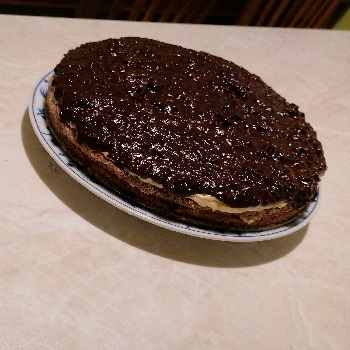
\includegraphics[height=5.5cm]{images/daim}
\def\portions{4}%
\textbf{{\normalsize Ingrediencie (\portions porcie):}}
%\vspace{0.5cm}
\begin{main}
	\item 150g fazuľa
	\item cibuľa
	\item bobkový list
	\item zemiaky
	\item smotana
	\item klobása
	\item červená paprika
	\item hladká múka
\end{main}
\end{ingredient}
\begin{recipe}
\textbf{{\normalsize Príprava:}}
\begin{enumerate}

\item{Deň vopred si fazuľu namočíme do vody (koľko vypije, toľko)}
\item{Uvaríme fazuľu s klobásou, bobkovým listom a cibuľou, osolíme}
\item{Keď je fazuľa skoro mäkká pridáme zemiaky}
\item{V smotane rozmiešame hladkú múku a červenú papriku}
\item{Zmiešame a necháme prevrieť}	

\end{enumerate}
\end{recipe}

\begin{notes}

\end{notes}
\clearpage	